\documentclass[12pt]{article}

\usepackage{graphicx}
\usepackage{paralist}
\usepackage{amsfonts}
\usepackage{amsmath}
\usepackage{hhline}
\usepackage{booktabs}
\usepackage{multirow}
\usepackage{multicol}
\usepackage{url}
\usepackage{hyperref}
\usepackage{graphicx}
\graphicspath{{}}

\oddsidemargin -10mm
\evensidemargin -10mm
\textwidth 160mm
\textheight 200mm
\renewcommand\baselinestretch{1.0}

\pagestyle {plain}
\pagenumbering{arabic}

\newcounter{stepnum}

%% Comments

\usepackage{color}

\newif\ifcomments\commentstrue

\ifcomments
\newcommand{\authornote}[3]{\textcolor{#1}{[#3 ---#2]}}
\newcommand{\todo}[1]{\textcolor{red}{[TODO: #1]}}
\else
\newcommand{\authornote}[3]{}
\newcommand{\todo}[1]{}
\fi

\newcommand{\wss}[1]{\authornote{blue}{SS}{#1}}

\title{Assignment 4 Specification}
\author{SFWR ENG 2AA4}

\begin {document}

\maketitle
This Module Interface Specification (MIS) document contains modules, types and
methods used for implementing the game 2048. At the start of the game, a board is created with two tiles 
in two random cells on the board containing a 2 or a 4 in each. The user must specify the direction that
the board shifts in order to merge the tiles that appear. When two tiles merge, their value get added 
together and leave behind a single tile instead. After a direction has been specified and the tiles
have been merged or moved in that direction, a new tile is added in a non-occupied spot containing a 2 or a
4. The possible directions are up ("w"), down ("s"), left ("a"), and right ("d"). This game play will continue
until there are no more places to add tiles and there are no possible merges, or when the player merges the 
tiles to create the value 2048. 

\begin{center}
	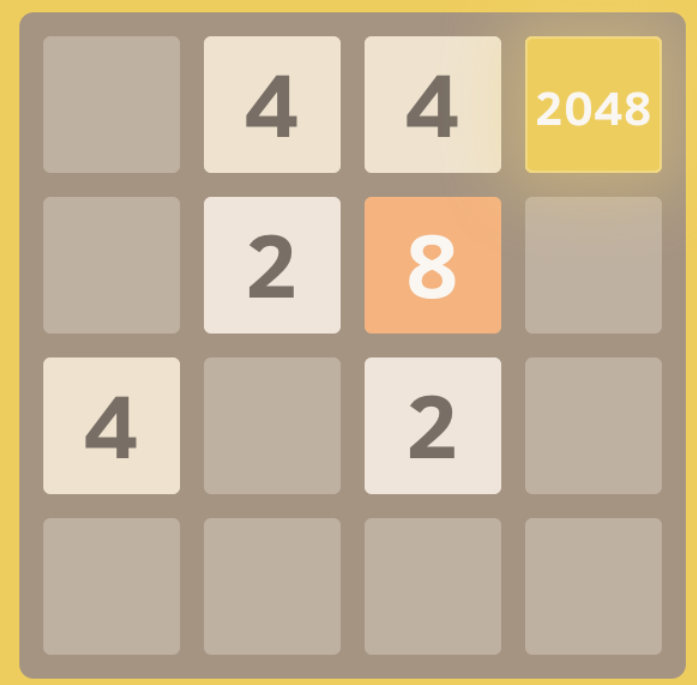
\includegraphics[scale=0.3]{2048_pic}
\end{center}

The above board visualization is from http://play2048.co/

\newpage

\section* {Overview of the design}

This design applies Module View Specification (MVC) design pattern and Singleton design pattern. The MVC components are 
$Play$ (controller module), $Board$ (model module) and $View$ (view module). The Singleton pattern is specified and 
implemented by $Play$ and $View$. 

A UML diagram is provided below for visualizing the structure of this software architecture:

\begin{center}
	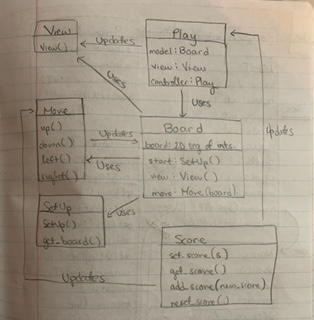
\includegraphics[scale=0.7]{image0}
\end{center}

The MVC design pattern is specified and implemented in the following way: the module $Board$ stores the current game board
state and the status of the game. It also allows for modifications to the current board state via its methods. A view module 
$View$ can display the state of the game board at a given time using text-based graphics printed to the user's console/screen. 
The controller $Play$ is responsible for handling input actions from the player, as well as displaying the rules and other 
messages for the user to see and interact with. 

For $Play$, they can get the score of the game by using the abstract method $Score.get_score()$ to check if the user has 
gotten to the value of 2048. 


\subsection* {Likely changes my design considers:}

\noindent Data structure for storing the game board.

\noindent Changes to the user input commands (play again ("y"), try again ("t") and keep going ("k")).

\noindent Changes to the scoring (input does not have to be power of 2 so could increase/decrease amount of points for high scores)

\newpage

\section* {SetUp Module}

\subsection*{Template Module}

SetUp

\subsection* {Uses}

None

\subsection* {Syntax}

\subsubsection* {Exported Constants}

None

\subsubsection* {Exported Types}

SetUp = ?

\subsubsection* {Exported Access Programs}

\begin{tabular}{| l | l | l | p{5cm} |}
\hline
\textbf{Routine name} & \textbf{In} & \textbf{Out} & \textbf{Exceptions}\\
\hline
new SetUp & & & \\
\hline
\end{tabular}

\subsection* {Semantics}

\subsubsection* {State Variables}

$\mathit{game\_board}: \text{grid}$

\subsubsection* {State Invariant}

None

\subsubsection* {Assumptions}

None

\subsubsection* {Access Routine Semantics}

\noindent new SetUp():
\begin{itemize}
\item transition: game\_board(random\_spot() = random\_num()), such that there are two unique cells filled once the transition is finished. 
\item output: $out := none$
\item exception: none
\end{itemize}

\noindent get\_board():
\begin{itemize}
\item output: $out := \mathit{gameboard}$
\item exception: none
\end{itemize}

\subsection*{Local Functions}

\noindent random\_num: \text{none} \rightarrow $\mathbb{N}$\\
\noindent $\mbox{random\_num}() \equiv \text{num} $
\textit{\# Where num is a random number such that a 2 is 90 percent likely, and 4 is 10 percent likely to occur} ~\\

\noindent random\_entry: \text{none} \rightarrow \text{seq of } $\mathbb{N}$\\
\noindent $\mbox{random\_entry}() \equiv \text{cell} $
\textit{\# Where cell is a random set of coordinates from a grid where each space in the grid is equally likely}$\\

\newpage

\section* {Score (Abstract Object)}

\subsection*{Module}

Score

\subsection* {Uses}

None

\subsection* {Syntax}

\subsubsection* {Exported Constants}

None

\subsubsection* {Exported Types}

Score = ?

\subsubsection* {Exported Access Programs}

\begin{tabular}{| l | l | l | p{5cm} |}
  \hline
  \textbf{Routine name} & \textbf{In} & \textbf{Out} & \textbf{Exceptions}\\
  \hline
  set\_score & $\mathbb{N}$ & & & \\
  \hline
  get\_score & & $\mathbb{N}$ & \\
  \hline
  add\_score & $\mathbb{N}$ & & \\
  \hline
  reset\_score & & & \\
  \hline
  
\end{tabular}

\subsection* {Semantics}

\subsubsection* {State Variables}

$\mathit{score}$: $\mathbb{N}$

\subsubsection* {State Invariant}

None

\subsubsection* {Assumptions}

The state variable will be set to zero (to start new score for game) before it is modified. It is also assumed that all inputs will be powers of $2$.

\subsubsection* {Access Routine Semantics}

\noindent set\_score($\mathit{s}$):
\begin{itemize}
\item transition: $\mathit{score} := \mathit{s}$
\item exception: none
\end{itemize}

\noindent get\_score( ):
\begin{itemize}
\item output: $out := \mathit{score}$
\item exception: none
\end{itemize}

\noindent add\_score(new_score):
\begin{itemize}
\item transition: $\mathit{score} := \mathit{score + new\_score}$
\item out: none
\item exception: none
\end{itemize}

\noindent reset\_score():
\begin{itemize}
\item transition: $\mathit{score} := 0$
\item out: none
\item exception: none
\end{itemize}

\newpage

\section* {Move}

\subsection*{Module}

Move

\subsection* {Uses}

Score

\subsection* {Syntax}

\subsubsection* {Exported Constants}

None

\subsubsection* {Exported Types}

Move = ?

\subsubsection* {Exported Access Programs}

\begin{tabular}{| l | l | l | p{5cm} |}
  \hline
  \textbf{Routine name} & \textbf{In} & \textbf{Out} & \textbf{Exceptions}\\
  \hline
  new Move & $\text{grid of } \mathbb{N})$ & & \\
  \hline
  up & & & \\
  \hline
  down & & & \\
  \hline
  left & & & \\
  \hline
  right & & & \\
  \hline
  
\end{tabular}

\subsection* {Semantics}

\subsubsection* {State Variables}

$\mathit{game\_board}$: $\text{grid of } \mathbb{N}$

\subsubsection* {State Invariant}

None

\subsubsection* {Assumptions}

Assumes the Board object that the Move class will be used in will be set up first before engaging in a move.  

\subsubsection* {Access Routine Semantics}

\noindent Move(board):
\begin{itemize}
\item transition: $\mathit{game\_board} := \mathit{board}$
\item out: none
\item exception: none
\end{itemize}

\noindent up( ):
\begin{itemize}
% NEED TO CHANGE INTO MATH
\item transition: \textit{\# Loop through board starting at second highest row and work towards last row. Check if cell above current cell has same value, if so merge(current, above cell). If cell above current cell is $0$, make above cell value the value of the current cell, current cell value now empty. Then after all cells have been shifted, add\_new\_block to game\_board} ~\\
\item exception: none
\end{itemize}

\noindent down( ):
\begin{itemize}
% NEED TO CHANGE INTO MATH
\item transition: \textit{\# Loop through board starting at second lowest row and work towards first row. Check if cell below current cell has same value, if so merge(current, below cell). If cell below current cell is $0$, make below cell value the value of the current cell, current cell value now empty. Then after all cells have been shifted, add\_new\_block to game\_board} ~\\
\item exception: none
\end{itemize}

\noindent left( ):
\begin{itemize}
% NEED TO CHANGE INTO MATH
\item transition: \textit{\# Loop through board starting at second leftmost row and work towards rightmost row. Check if cell to left of current cell has same value, if so merge(current, left cell). If cell left of current cell is $0$, make left cell value the value of the current cell, current cell value now empty. Then after all cells have been shifted, add\_new\_block to game\_board} ~\\
\item exception: none
\end{itemize}

\noindent right( ):
\begin{itemize}
% NEED TO CHANGE INTO MATH
\item transition: \textit{\# Loop through board starting at second rightmost row and work towards leftmost row. Check if cell to right of current cell has same value, if so merge(current, right cell). If cell right of current cell is $0$, make right cell value the value of the current cell, current cell value now empty. Then after all cells have been shifted, add\_new\_block to game\_board} ~\\
\item exception: none
\end{itemize}

\subsection*{Local Functions}

\noindent merge: \text{seq of } $\mathbb{N}, \text{seq of } $\mathbb{N} \rightarrow none \\
\noindent $\mbox{merge}(cell1, cell2) \equiv \text{merge} $
\textit{\# Where merge changes the cell1 to a value of $0$, and doubles the value of cell2, while adding the value in cell2 to the Score abstract object} ~\\

\noindent add\_new\_block: none \rightarrow none \\
\noindent $\mbox{add\_new\_block}() \equiv \text{add} $
\textit{\# Where add adds another random number in a random empty spot on the game board, if no spot is free, do not add block} ~\\

\noindent random\_num: \text{none} \rightarrow $\mathbb{N}$\\
\noindent $\mbox{random\_num}() \equiv \text{num} $
\textit{\# Where num is a random number such that a 2 is 90 percent likely, and 4 is 10 percent likely to occur} ~\\

\noindent random\_entry: \text{none} \rightarrow \text{seq of } $\mathbb{N}$\\
\noindent $\mbox{random\_entry}() \equiv \text{cell} $
\textit{\# Where cell is a random set of coordinates from a grid where each space in the grid is equally likely}~\\

\newpage

\section* {Board (ADT)}

\subsection*{Module}

Board

\subsection* {Uses}

SetUp, View, Move

\subsection* {Syntax}

\subsubsection* {Exported Constants}

None

\subsubsection* {Exported Types}

Board = ?

\subsubsection* {Exported Access Programs}

\begin{tabular}{| l | l | l | p{5cm} |}
  \hline
  \textbf{Routine name} & \textbf{In} & \textbf{Out} & \textbf{Exceptions}\\
  \hline
  start & & & & \\
  \hline
  view & & & \\
  \hline
  move & String & & \\
  \hline
  get\_board & & $\text{seq of (seq of) } \mathbb{N}$ & \\
  \hline
  get\_board\_value & $\mathbb{N}, \mathbb{N}$ & $\mathbb{N}$ & \\
  \hline
  
\end{tabular}

\subsection* {Semantics}

\subsubsection* {State Variables}

$\mathit{game\_board}$: $\text{sequence [] } \mathbb{N}$

\subsubsection* {State Invariant}

game_board[i][j] = [4][4]  \textit{\# Size of the board is 4x4}~\\\

\subsubsection* {Assumptions}

Move input (direction) assumed to be only "wasd" characters. 

\subsubsection* {Access Routine Semantics}

\noindent start( ):
\begin{itemize}
\item transition: $\mathit{game\_board} := \mathit{SetUp.get\_board()}$
\item out: none
\item exception: none
\end{itemize}

\noindent view( ):
\begin{itemize}
\item transition: \textit{\# New instance of View(game\_board) to show player the state of the board}~\\\
\item exception: none
\end{itemize}

\noindent move( ):
\begin{itemize}
\item transition: \textit{\# New instance of Move(game\_board)}~\\

$(\langle direction = "w" \rightarrow Move.up() | direction = "s" \rightarrow Move.down() | direction = "a" \rightarrow Move.left() | True \rightarrow Move.right()) \rangle$

\item exception: none
\end{itemize}

\noindent get\_board( ):
\begin{itemize}
\item out: $\mathit{game\_board}$
\item exception: none
\end{itemize}

\noindent get\_board\_value(i, j):
\begin{itemize}
\item out: $\mathit{game\_board[i][j]}$
\item exception: none
\end{itemize}

\newpage

\section* {View Module}

\subsection* {Module}

View

\subsection* {Uses}

Score

\subsection* {Syntax}

\subsubsection* {Exported Types}

View = ?

\subsubsection* {Exported Access Programs}

\begin{tabular}{| l | l | l | l |}
\hline
\textbf{Routine name} & \textbf{In} & \textbf{Out} & \textbf{Exceptions}\\
\hline
new View & $\text{grid of } \mathbb{N})$ & & \\
\hline

\end{tabular}

\subsection* {Semantics}

\subsubsection* {Environmental Variables}

window: A portion of the computer screen that displays the game and messages. 

\subsubsection* {State Variables}

None

\subsubsection* {State Invariant}

None

\subsubsection* {Assumptions}

None

\subsubsection* {Access Routine Semantics}

\noindent View(game\_board)

\begin{itemize}
\item transition: $\mathit{window} := \mathit{Displays Score using Score abstract object, displays all cells in game\_board}$

\end{itemize}

\newpage

\section* {Critique of Design}

\begin{itemize}

\item The design was consistent in how the functions were able to be used in a consistent way in the Board class. Also the
naming of game\_board variables was consistent, as well as ways to access this variable across all modules that invloved it.

\item Some methods like get\_score, get\_board and get\_board\_value are not essential in order for the game to work, but allowed ease of use when accessing this information from other classes to help get the status of the game more easily. 

\item The methods up(), down(), left() and right() in the Move class are minimal as they allow movement in each specific direction as opposed to be able to move in all the different ways using one method. This allows for better usability as the programmer knows exactly which method moves which way and if they wanted to change the functionality of a certain direction only then this would allow them to do so. It also allows for better readibility as any future programmers that may read it know how each direction will function in that method. 

\item The View method allows for some generality as it does not specify the size of the board that is being printed for the user, it just prints based on the length of the first row. This means that any square board would be able to be printed out using this method. This is also true in the Board class, however the SetUp and move methods are specified for a 4x4 grid. This could be changed to be more general design if there was an input in the SetUp constructor that allowed for the changing of the size of the grid to fit the input paramaters, and in the Move method in the loops instead of specifying the loop stop when i less than 4 which is the length of the grid, that could have been changed to simply the length of the rows for i and length of columns for j to be checked instead. 

\item This design was not general in its implementation of the controls as the user can only use "wasd" to play instead of also being able to use the arrow keys or "ijkl" is they wanted to. A way to fix this to make it more general is to ask the user before the game starts to input four characters that they would like to use to control the game which would then be incorporated into the controls. 

\item This design has high cohesion as all the modules relate to each other as a result of MVC. For example, Score is used in Move, Board and View, and SetUp, Move and View being used in Board. All of these methods working together allow the game to function and it would not be able to function correctly if one of them was not working correctly, as they are all essential to making the Play function work and allowing the user to play the game. 

\item I specified Board module as an ADT as it makes it easier to create a new Board object when restarting a game. 

\item The score was implemented as an abstract object as it allowed the Score to be updated and used from any class when 
needed, which allowed for ease of use in accessing the score of the current game. 

\item The testing of these methods were made to try to prove the correctness of the modules and their methods. This was done by testing each method in a variety of ways to be able to catch any errors that may have arisen from that process. The testing allowed for the game to be played so that the user does not need to worry about the game crashing from an incorrect input. This was done in the Play method as if the user entered an incorrect input, the program would ask the user to try again until their input was correct. 

\item This design supports information hiding as there is no way to modify the SetUp or View methods, as well as the state variables for Move and Board. This allows the main board that the user is playing on to be private and keep the user from cheating. However, the Score method can be set to a different score at any time using its setter methods but that does not guarntee the win condition, only that they have a higher score for the leader boards. The win condition is also hidden from the user and cannot be modified, but a way to make this even more hidden is if it as inside a Check\_Win class instead of the method in Play, as then the user would have a harder time finding the win condition. 

\end{itemize}

\newpage

\section* {Answers to Questions}

\item 1. UML diagram for modules in $A3$

\begin{figure}[ht]
\centering
\begin{minipage}[b]{0.45\linewidth}
	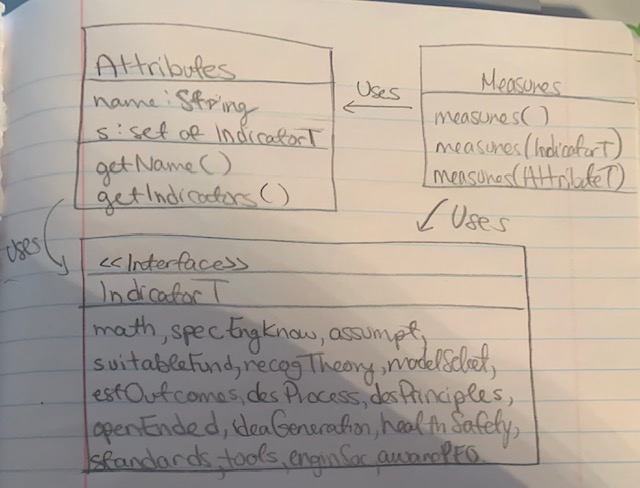
\includegraphics[scale=0.3]{IMG_3018}
\end{minipage}
	\quad
\begin{minipage}[b]{0.45\linewidth}
	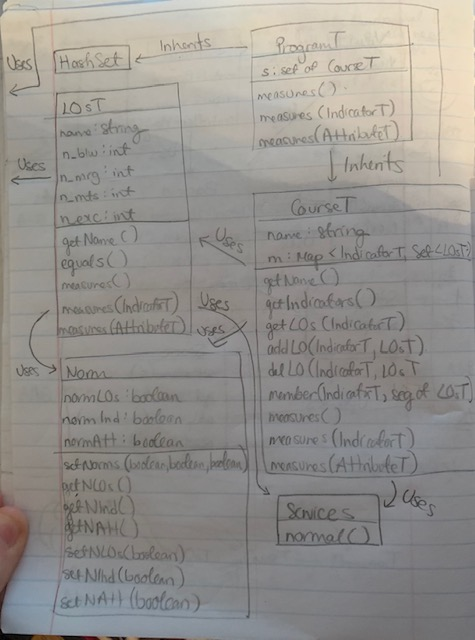
\includegraphics[scale=0.3]{IMG_3017}
\end{minipage}
\end{figure}

\noindent where LOsT and CourseT use Measures (it was hard to try to line up)

\item 2. Convex Hull Control Flow Graph

\begin{center}
	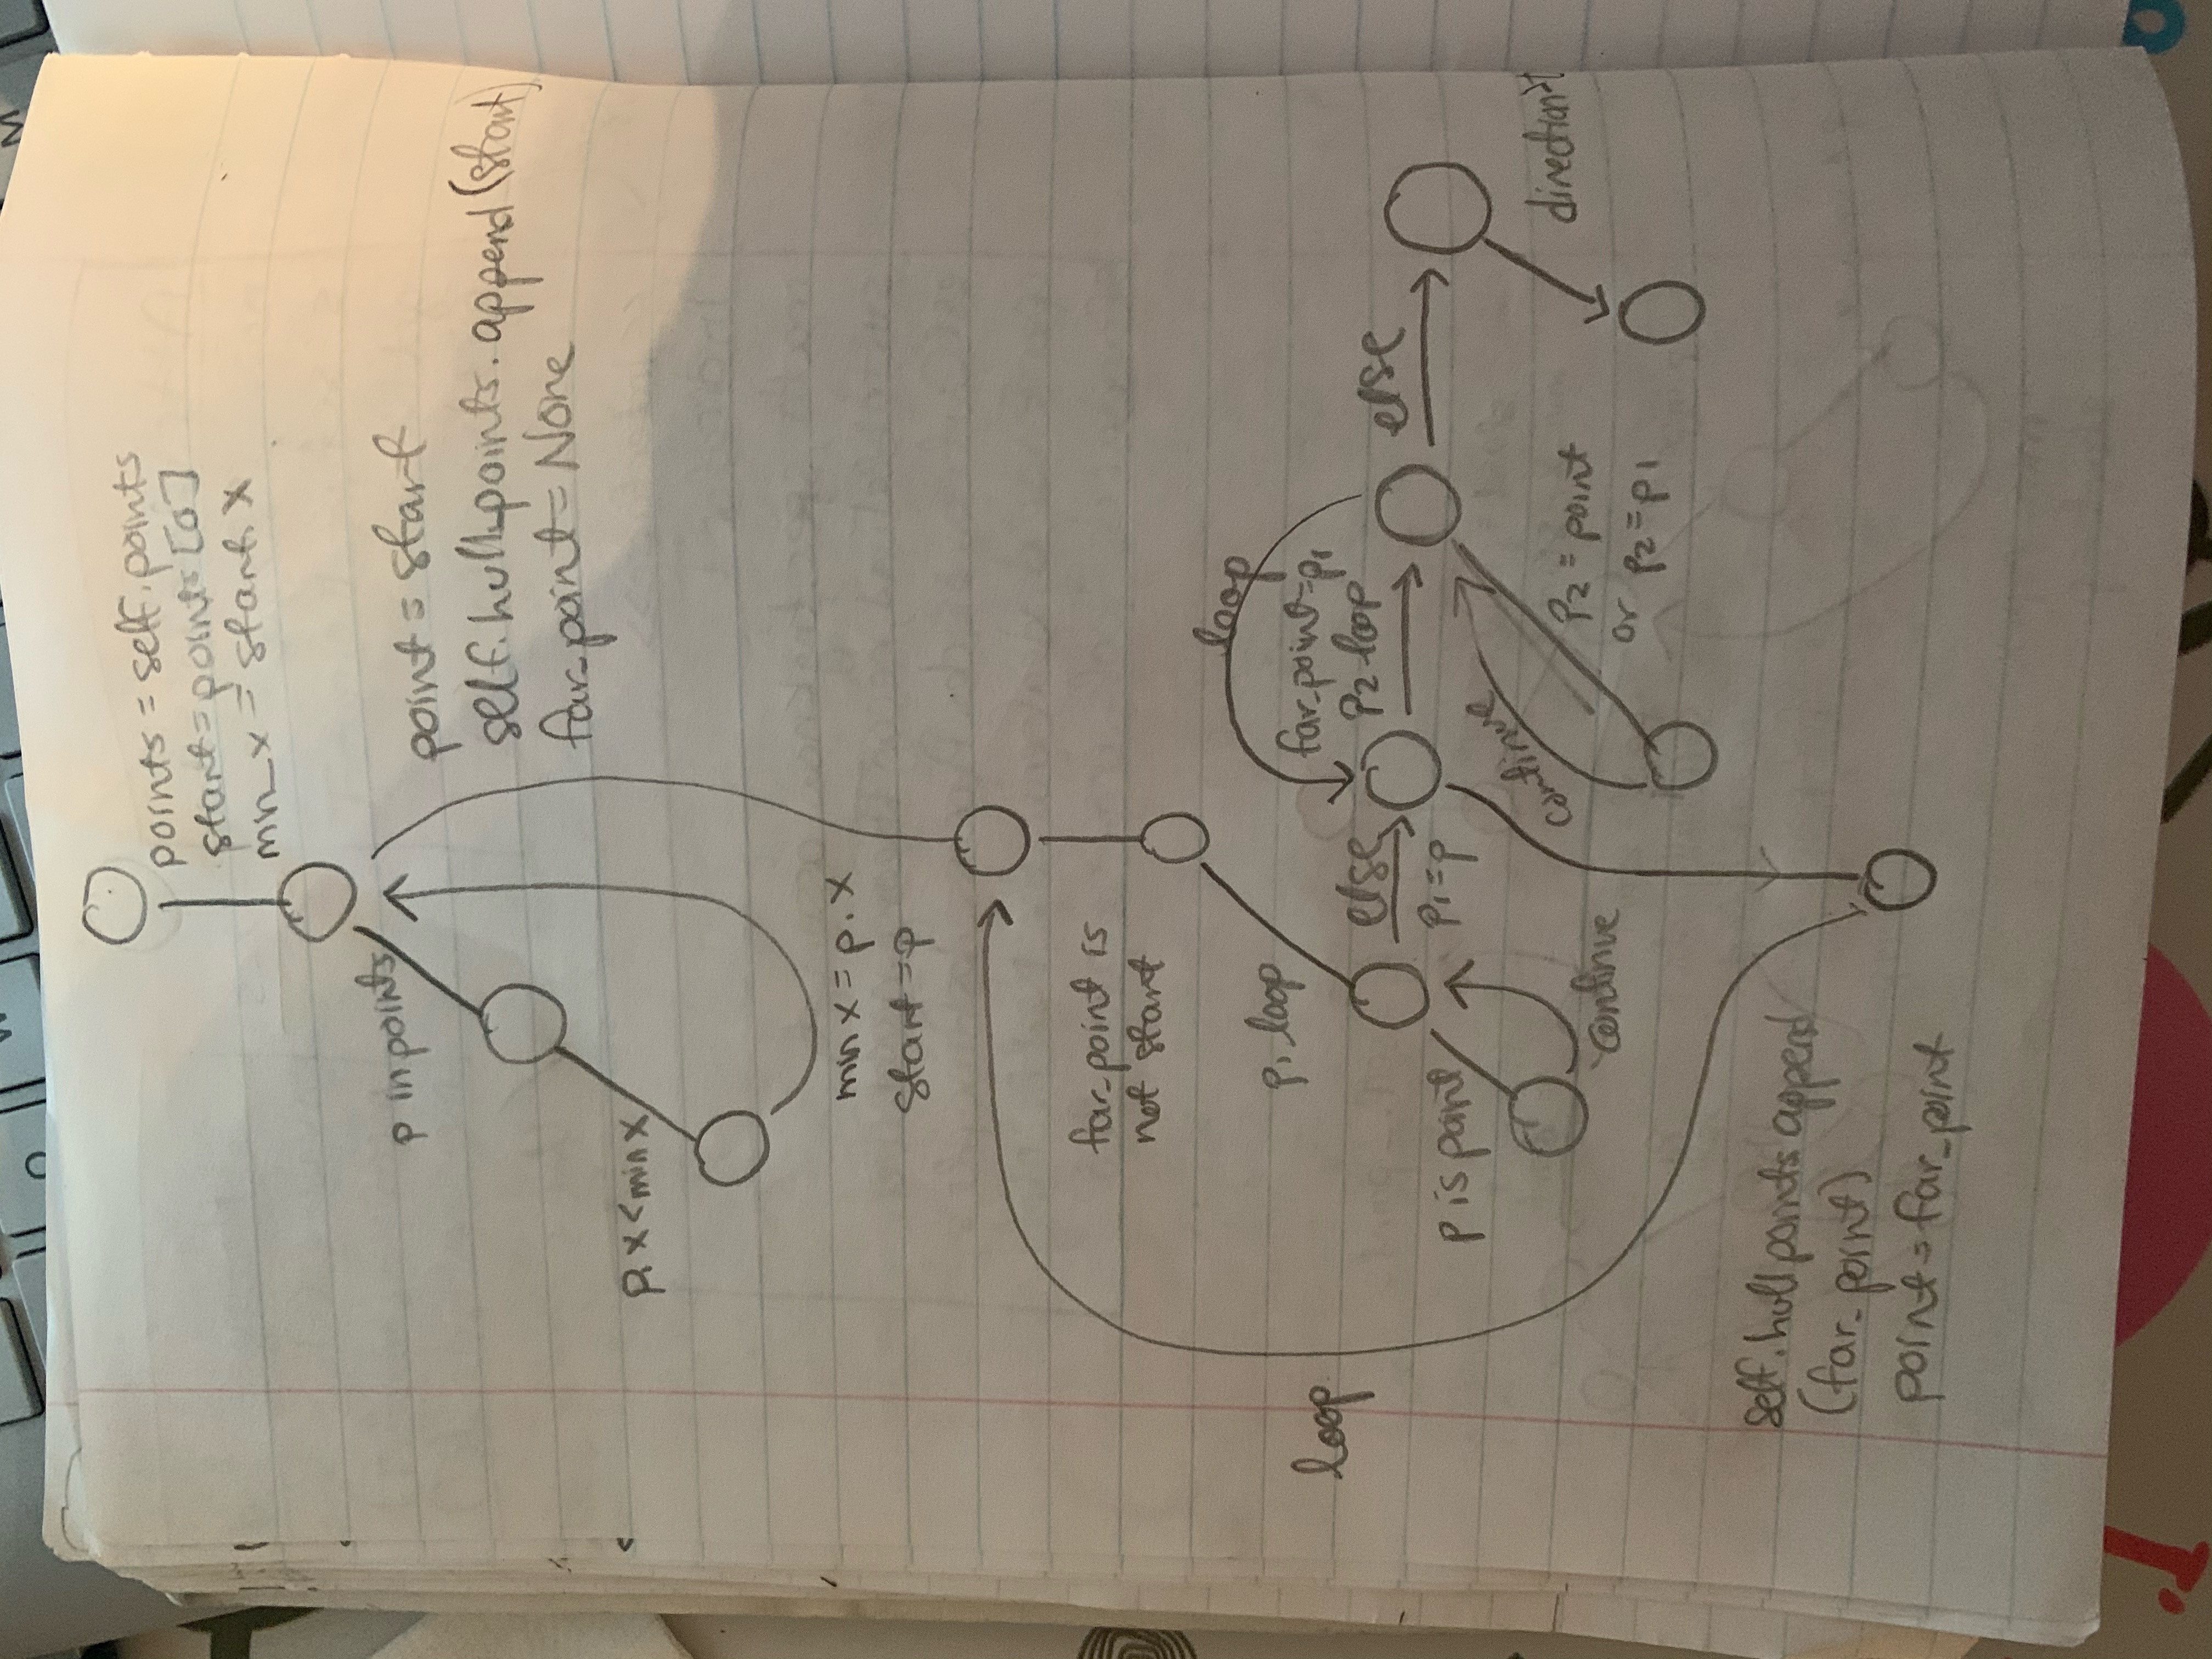
\includegraphics[scale=0.1]{Flow}
\end{center}

\end {document}
